\chapter{Methodology}\label{ch:methodology}

\section{Introduction}\label{sec:intro}

In this chapter, the development process for \textbf{Collective} mobile journaling application is explained using the Rapid Application Development (RAD) methodology. Each stage of the developemnt is explained in detail, covering the phases of requirements planning, user design, construction and cutover.

\section{Rapid Application Development (RAD) Methodology}\label{sec:rad}

\begin{figure}[H]
\centering
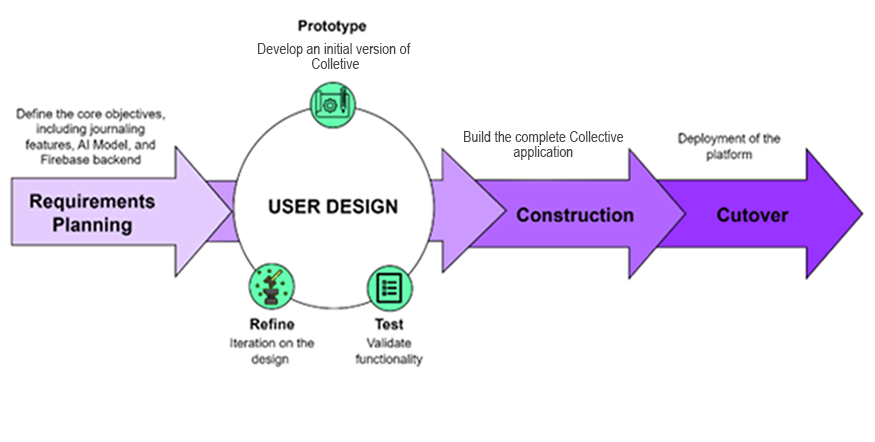
\includegraphics[width=0.8\textwidth]{files/imgs/RAD.png}
\caption{Rapid Application Development (RAD) Methodology Phases}
\label{fig:rad-methodology}
\end{figure}

Rapid Application Development (RAD) is a software development methodology that emphasizes quick development and iteration of prototypes over rigorous planning and testing. It is particularly useful for projects where requirements are expected to evolve or are not fully understood at the outset. The RAD methodology consists of four main phases: requirement planning, user design, construction, and cutover. This model was chosen for the development of the \textbf{Collective} mobile journaling application due to its flexibility and focus on user feedback, which is crucial for creating a user-friendly and effective application. The detais of the project is discussed below:

\section{Requirement planning}\label{sec:requirementPlanning}   

The requirement planning phase is the first step in the RAD methodology, where the project team identifies and defines the requirements of the application. This phase involves gathering information from stakeholders, including potential users, to understand their needs and expectations. The goal is to create a clear and concise set of requirements that will guide the development process.

\subsection{Software Requirements}\label{subsec:softwareRequirements}

The following tables list the software and tools used to develop the \textbf{Collective} mobile journaling application:

\begin{table}[H]
\centering
\caption{Visual Studio Code}
\label{tab:vscode-metadata}
\begin{tabular}{|p{4cm}|p{10cm}|}
\hline
\textbf{Attribute} & \textbf{Details} \\
\hline
Name & Visual Studio Code \\
\hline
Mnemonic & VS Code \\
\hline
Specification Number & N/A \\
\hline
Version Number & 1.101.1 \\
\hline
Source & \url{https://code.visualstudio.com/} \\
\hline
\end{tabular}
\end{table}

\begin{table}[H]
\centering
\caption{Flutter}
\label{tab:flutter-metadata}
\begin{tabular}{|p{4cm}|p{10cm}|}
\hline
\textbf{Attribute} & \textbf{Details} \\
\hline
Name & Flutter \\
\hline
Mnemonic & Flutter SDK \\
\hline
Specification Number & N/A \\
\hline
Version Number & 3.10.0 \\
\hline
Source & \url{https://flutter.dev/} \\
\hline
\end{tabular}
\end{table}

\begin{table}[H]
\centering
\caption{Dart}
\label{tab:dart-metadata}
\begin{tabular}{|p{4cm}|p{10cm}|}
\hline
\textbf{Attribute} & \textbf{Details} \\
\hline
Name & Dart \\
\hline
Mnemonic & Dart SDK \\
\hline
Specification Number & N/A \\
\hline
Version Number & 3.0.0 \\
\hline
Source & \url{https://dart.dev/} \\
\hline
\end{tabular}
\end{table}

\begin{table}[H]
\centering
\caption{Google Chrome}
\label{tab:chrome-metadata}
\begin{tabular}{|p{4cm}|p{10cm}|}
\hline
\textbf{Attribute} & \textbf{Details} \\
\hline
Name & Google Chrome \\
\hline
Mnemonic & Chrome Browser \\
\hline
Specification Number & N/A \\
\hline
Version Number & 114.0.5735.199 \\
\hline
Source & \url{https://www.google.com/chrome/} \\
\hline
\end{tabular}
\end{table}

\begin{table}[H]
\centering
\caption{Microsoft Word}
\label{tab:msword-metadata}
\begin{tabular}{|p{4cm}|p{10cm}|}
\hline
\textbf{Attribute} & \textbf{Details} \\
\hline
Name & Microsoft Word \\
\hline
Mnemonic & MS Word \\
\hline
Specification Number & N/A \\
\hline
Version Number & Office 365 \\
\hline
Source & \url{https://www.microsoft.com/en-us/microsoft-365/word} \\
\hline
\end{tabular}
\end{table}

\begin{table}[H]
\centering
\caption{Microsoft Excel}
\label{tab:msexcel-metadata}
\begin{tabular}{|p{4cm}|p{10cm}|}
\hline
\textbf{Attribute} & \textbf{Details} \\
\hline
Name & Microsoft Excel \\
\hline
Mnemonic & MS Excel \\
\hline
Specification Number & N/A \\
\hline
Version Number & Office 365 \\
\hline
Source & \url{https://www.microsoft.com/en-us/microsoft-365/excel} \\
\hline
\end{tabular}
\end{table}

\begin{table}[H]
\centering
\caption{Draw.io}
\label{tab:drawio-metadata}
\begin{tabular}{|p{4cm}|p{10cm}|}
\hline
\textbf{Attribute} & \textbf{Details} \\
\hline
Name & Draw.io \\
\hline
Mnemonic & Diagram Tool \\
\hline
Specification Number & N/A \\
\hline
Version Number & 20.8.0 \\
\hline
Source & \url{https://app.diagrams.net/} \\
\hline
\end{tabular}
\end{table}

\begin{table}[H]
\centering
\caption{DeepSeek API}
\label{tab:deepseek-metadata}
\begin{tabular}{|p{4cm}|p{10cm}|}
\hline
\textbf{Attribute} & \textbf{Details} \\
\hline
Name & DeepSeek API \\
\hline
Mnemonic & DeepSeek \\
\hline
Specification Number & N/A \\
\hline
Version Number & DeepSeek-V3-0324 \\
\hline
Source & \url{https://platform.deepseek.com/} \\
\hline
\end{tabular}
\end{table}

\subsection{Hardware Requirements}\label{subsec:hardwareRequirements}

The following table lists the hardware requirements necessary for the development and testing of the \textbf{Collective} mobile journaling application. Note that the development is currently focused exclusively on the Android platform, as iOS development requires a macOS machine, which is planned for future work:

\begin{table}[H]
\centering
\caption{Hardware Requirements}
\label{tab:hardware-requirements}
\begin{tabular}{|p{4cm}|p{10cm}|}
\hline
\textbf{Component} & \textbf{Specification} \\
\hline
Processor & Intel Core i5 or equivalent \\
\hline
RAM & 8 GB or higher \\
\hline
Storage & 256 GB SSD or higher \\
\hline
Operating System & Windows 10 \\
\hline
Additional Devices & Android smartphone for testing \\
\hline
\end{tabular}
\end{table}

\subsection{Use Case Diagram}\label{subsec:usecaseDiagram}

The use case diagram for the \textbf{Collective} mobile journaling application illustrates the interactions between the user (Writer) and the system. It highlights the various functionalities provided by the application and their relationships. The diagram is shown below:

\begin{figure}[H]
\centering
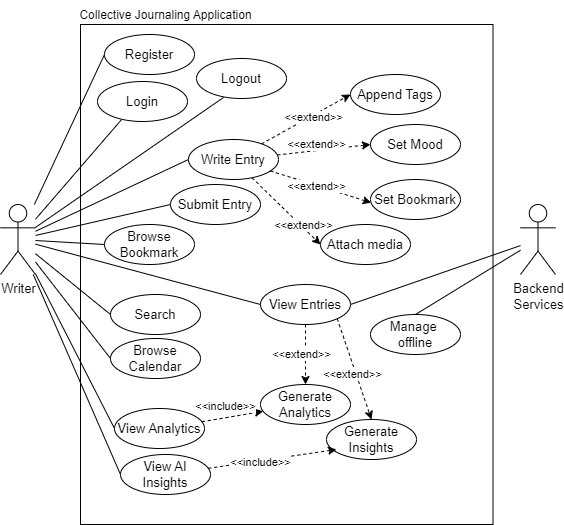
\includegraphics[width=0.8\textwidth]{files/imgs/usecase_diagram.png}
\caption{Use Case Diagram for Collective Mobile Journaling Application}
\label{fig:usecase-diagram}
\end{figure}

\subsection{Use Case Description}\label{subsec:usecaseDescription}

The use case description provides detailed information about the functionalities depicted in the use case diagram. Below is a table summarizing the key use cases:

\begin{table}[H]
\centering
\caption{Use Case Description}
\label{tab:usecase-description}
\begin{tabular}{|p{4cm}|p{6cm}|p{6cm}|}
\hline
\textbf{Actor} & \textbf{Use Case} & \textbf{Use Case Description} \\
\hline
\multirow{15}{*}{Writer} & Register & Allows the user to create an account. \\
\cline{2-3}
 & Login & Allows the user to log in to the application. \\
\cline{2-3}
 & Logout & Allows the user to log out when done. \\
\cline{2-3}
 & Write Entry & Enables the user to compose journal entries. \\
\cline{2-3}
 & Append Tags & Allows the user to add tags to journal entries. \\
\cline{2-3}
 & Set Mood & Enables the user to set mood for journal entries. \\
\cline{2-3}
 & Set Bookmark & Allows the user to bookmark entries. \\
\cline{2-3}
 & Attach Media & Enables the user to attach media to entries. \\
\cline{2-3}
 & Submit Entry & Allows the user to submit journal entries. \\
\cline{2-3}
 & Browse Bookmark & Enables the user to browse bookmarked entries. \\
\cline{2-3}
 & View Entries & Allows the user to browse through saved entries. \\
\cline{2-3}
 & Search & Enables the user to search entries. \\
\cline{2-3}
 & Browse Calendar & Allows the user to view entries by calendar. \\
\cline{2-3}
 & View Analytics & Provides tools to analyze journal entries. \\
\cline{2-3}
 & View AI Insights & Offers AI-based insights for journal entries. \\
\hline
\multirow{4}{*}{Backend Services} & View Entries & Handles data storage and retrieval for entries. \\
\cline{2-3}
 & Manage Offline & Provides functionality to access entries offline. \\
\cline{2-3}
 & Generate Analytics & Offers tools to analyze journal entries. \\
\cline{2-3}
 & Generate Insights & Provides insights based on journal entries. \\
\hline
\end{tabular}
\end{table}

\section{User design}\label{sec:userDesign}